\subsection{Descripción del problema.}

\vspace*{0.3cm}

Nuestro país está infectado de zombies y nosotros debemos idear un plan estratégico para retomar el poder del mismo. Debido a que los zombies pudieron no haber invadido solo nuestro territorio, dejaremos un legado a la humanidad en forma de algoritmo, para que en un futuro, la humanidad recobre el poder.
%%si no les gusta esta versión, la anterior y aburrida empezaba aca, salvo que la primer oración era: tenemos un pais infectado de zombies.(ALE)
Entonces, nos enfocaremos en ver como salvar un país.Un país esta dividido en ciudades. Nuestro objetivo es salvar la mayor cantidad de ciudades de este país, enviando soldados a ellas. Una ciudad se considera salvada si los soldados exterminan todos los zombies de dicha ciudad.

Aspectos a tener en cuenta:

\begin{itemize}
   \item Los recursos del país son acotados.
   \item Se conoce la cantidad de ciudades del país, y estas tienen un orden.
   \item Se conoce la cantidad de soldados atrincherados en cada ciudad (soldados iniciales de la ciudad).
   \item Se conoce la cantidad de zombies en cada ciudad.
   \item Para cada ciudad, se conoce el costo de enviar un soldado.
   \item Cada soldado se puede encargar como máximo de 10 zombies.
   \item la complejidad del algoritmo propuesto debe ser $\mathcal{O}(n*log(n))$.
	\item Siendo una situación tan crítica, el orden es importante, por lo que este algoritmo proveera la siguiente salida:

$C$ $s_{1}$ $s_{2}$ ... $s_{n}$

donde $C$ es la cantidad de ciudades que se podrían recuperar siguiendo la solución y, suponiendo que el país tiene $n$ ciudades, $s_{1}$, ..., $s_{n}$ son las cantidades de soldados de refuerzo que deberían enviarse a cada una de las ciudades de la instancia. Es decir, a la ciudad $i$ se enviaran $s_{i}$ soldados de refuerzo (las ciudades se numeran de 1 a n segun el orden)
%%no se como disfrazar al orden dado por la entrada, porque es importante, hablo de la entrada tambien, o no??(ALE)
\end{itemize}

Ejemplo:

Supongamos un país con 3 ciudades y un presupuesto de 50.

Las características de las ciudades son las siguientes:
\begin{itemize}
	\item La ciudad 1 tiene 15 zombies, 0 soldados atrincherados, y un costo por enviar un soldado de 10.
	\item La ciudad 2 tiene 77 zombies, 6 soldados atrincherados, y un costo por enviar un soldado de 20.
	\item La ciudad 3 tiene 425 zombies, 13 soldados atrincherados, y un costo por enviar un soldado de 1.
\end{itemize}

En este caso, se salvarían las ciudades 1 y 3, dado que el presupuesto no alcanza para salvar a las tres ciudades, y que si se salva la ciudad 2, se gasta 40, y con los 10 que quedan no se pueden salvar ninguna de las dos ciudades restantes.

Veamos que, si el costo por enviar un soldado de la ciudad 2 fuera de 10, no se podrían salvar las tres ciudades, pero se podrían salvar dos, y habría que elegir entre las tres ciudades, dos para salvar.

%\begin{figure}[htb]
%  \begin{center}
%      \includegraphics[scale=0.25]{imagenes/ejemplo.jpg}
%  \end{center}
%  \caption{ejemplo}
%\end{figure}
\vspace*{0.6cm}
%\newpage
\subsection{Desarrollo de la idea.}

\vspace*{0.3cm}

Notemos que para recuperar la mayor cantidad de ciudades de un país en manos de los zombies, nosotros lo único que podemos hacer es enviar soldados a sus ciudades teniendo en cuenta la cantidad de soldados que esta ciudad posee de por sí. Como esto es la guerra, no tiene ningún sentido enviar soldados a una ciudad sino estamos seguros de que ésta se salvará, puesto que es un desperdicio de presupuesto y vidas humanas. Por otro lado, debido a que queremos salvar la mayor cantidad de ciudades, y sabemos que para salvar una ciudad necesitamos como MÍNIMO 1 soldado por cada diez zombies, si enviamos soldados a una ciudad, nos aseguraremos de enviar la menor cantidad de soldados posibles, así ahorramos recursos que podrán ser utilizados en otra ciudad. Tomando en cuenta todo lo antes dicho, para resolver este problema, la idea será primero tener conocimiento de cuánto cuesta salvar cada ciudad. Para esto, basta hacer la siguiente cuenta por cada ciudad: %(las variables abajo expuestas no pertenecen al algoritmo, son simplemente a modo de ayuda para entender que se hace):
\begin{itemize}
   \item $zombis.vivos = zombis.totales - 10 * soldados.atrincherados.de.la.ciudad$
   \item $soldados.requeridos = \left \lceil \dfrac{zombis.vivos}{10} \right \rceil$ (redondeado hacia arriba, puesto que no puedo enviar medio soldado)
   \item $costo.salvacion.de.la.ciudad = soldados.requeridos * costo.por.soldado.de.la.ciudad$
\end{itemize}

Luego de calcular estos valores, se ordenarán las ciudades de menor a mayor respecto a su costo para ser salvadas y, de manera golosa, irlas salvando en ese orden hasta cubrir el presupuesto.

%\begin{codebox}
%\Procname{$\proc{ejemplo_de_pseudocodigo}(x,y)$}
%\li \Return $\id{solucion}$
%\end{codebox}

\vspace*{0.6cm}

%\newpage
\subsection{Demostración de correctitud.}

\vspace*{0.3cm}

Tenemos dos casos:
\begin{enumerate}
	\item No se salva ninguna ciudad
	\item Se salva al menos una ciudad
\end{enumerate}

\subsubsection{No se salva ninguna ciudad:}

No se salva nadie $\Longleftrightarrow$ nuestro algoritmo dice que no se salva nadie.

$\Longrightarrow )$ Supongamos que no se salva nadie, eso quiere decir que no existe ninguna ciudad tal que si yo gasto todo mi presupuesto en enviarle soldados, ésta obtenga 1 soldado por cada 10 zombies como mínimo.

Sea $p$ un presupuesto tal que no llegue a cumplir los costos de envío de soldados mínimo para salvar ninguna ciudad.
Particularmente, si $p$ no alcanza para salvar a ninguna ciudad, no alcanza para salvar a la ciudad que menos presupuesto necesita para ser salvada (si hay más de una cuyo costo es el mínimo, en particular no se puede salvar ninguna de ellas).$(A)$

Por lo tanto, cuando mi algoritmo ordene las ciudades por costo de salvación, que es justamente el costo que tiene conseguir la mínima cantidad de soldados necesarios para salvar esa ciudad, y tome la primer ciudad, que es la que menos costo tiene para ser salvada (o por lo menos una de ellas), por lo dicho en $(A)$, el algoritmo no tomará esta ciudad ya que el presupuesto no alcanza, y devolverá que se pueden salvar 0 ciudades, y no enviará tropas, el país está perdido, fracasamos, NO SE SALVA NADIE.

$\Longleftarrow )$ Supongamos que nuestro algoritmo dice que no se salva nadie.

Eso significa que por lo explicado anteriormente, el presupuesto es menor a la ciudad que menos costo tiene para ser salvada (si hay varios mínimos, esto no molesta ya que justamente tienen el mismo costo por salvación).

Pero si el presupuesto es menor al costo de salvar a la ciudad (o ciudades) que menos dinero requiere por salvarse, entonces el presupuesto es menor al costo de salvar cualquier ciudad.

Si el presupuesto no alcanza para salvar ninguna ciudad, entonces nuevamente, NO SE SALVA NADIE.

\subsubsection{Se salva al menos una ciudad:}

Hay solución no vacía $\Longleftrightarrow$ nuestro algoritmo devuelve solución óptima.

Sea $N$ nuestra solución óptima, la solución armada con el algoritmo goloso, y $O$ la solución óptima que más se parece a $N$. Asumimos $N$ no óptima y ordenamos $O$ por el costo de salvación, de menor a mayor.
Sea $N_{k}$ el primer elemento en el que $N$ difiere de $O$, o sea $\forall i<k , N_{i}=O_{i}$.

Dado que $N_{k}$ fue obtenido usando el algoritmo goloso sabemos que $Costo(N_{k}) \geq Costo(N{k-1})$ y que $\forall j>k, Costo(N_{k}) \leq Costo(N_{j})$.

En otras palabras, $Costo(N_{k})$ es el menor de todas los costos por salvación mayores a $Costo(N_{k-1})$. Por lo tanto $Costo(N_{k}) \leq Costo(O_{k})$, luego puedo reemplazar $O_{k}$ por $N_{k}$ y obtengo una solución óptima que se parece más que la $O$ original a $N$. ABSURDO puesto que partimos de que $O$ es la solución óptima que más se parece a $N$.

Este absurdo viene de suponer que $N$ no es óptima.  Entonces podemos concluír que, si existe alguna solución, nuestro algoritmo goloso obtiene la solución óptima.

\vspace*{0.6cm}

%\newpage
\subsection{Análisis de complejidad.}

\vspace*{0.3cm}

A continuación mostraremos que la complejidad total de nuestro algoritmo es $\mathcal{O}(n*log(n))$.

Primeramente, veamos la complejidad de la parte golosa (Figura \ref{code:goloso}).  Las primeras dos líneas son asignaciones, así que cuentan como $\mathcal{O}(1)$. En la línea 3 comienza un ciclo que recorrerá las ciudades (previamente ordenadas por costo de salvación) hasta que se supere el presupuesto o se terminen de ver las ciudades. Dentro de ese ciclo, se va acumulando el costo de salvar la ciudad, y en caso de estar dentro del presupuesto, se la salva.  La línea 6 será sólo una asignación a una variable que determinará que dicha ciudad será salvada, así que como sólo tenemos una comparación, un incremento y a lo sumo dos asignaciones, cada iteración del ciclo tendrá una complejidad de $\mathcal{O}(1)$.  Como el ciclo itera a lo sumo n veces, podemos decir que esta parte tiene complejidad $\mathcal{O}(n)$.

\begin{figure}[!ht]
\begin{codebox}
\Procname{int $\proc{zombie_goloso}(lista$_$ciudades, int$ $n, int$ $p)$}
\li i $\leftarrow$ 0
\li sum $\leftarrow$ 0
\li \While ($i<n$ y $sum \leq p$) 
\li 		\Do   
		$sum$ + costo_salvar_ciudad_i   
\li		\If $sum<p$
\li 			\Then salvar_ciudad_i
\li				$i++$
			\End
	\End
\li \Return $\id{i}$       
\end{codebox} 
\caption{Pseudocódigo del algoritmo goloso}\label{code:goloso}
\end{figure}
\FloatBarrier

Analicemos ahora la complejidad del algoritmo completo (Figura \ref{code:zombieland}). Las primeras dos líneas son lecturas de datos, las cuales pueden considerarse $\mathcal{O}(1)$.  En la línea 3 se crea una lista con las n ciudades indicadas; si consideramos $\mathcal{O}(1)$ la creación de una lista vacía y $\mathcal{O}(1)$ la lectura y escritura de cada una de las ciudades, podemos decir que este paso es $\mathcal{O}(n)$.  La línea 4 calcula el costo de salvar cada ciudad, para lo cual se recorre toda la lista de ciudades y se hacen los cálculos previamente descritos, así que nuevamente tenemos una complejidad de $\mathcal{O}(n)$.  Luego, en la línea 5, pasamos a ordenar las ciudades por ese costo de salvación, y sabemos que este ordenamiento puede ser implementado con una complejidad de $\mathcal{O}(n*log(n))$. Acto seguido, se hace el llamado a la función golosa analizada anteriormente ($\mathcal{O}(n)$) y se vuelve a ordenar la lista, esta vez por el nombre (un número) que identifica a cada ciudad según el orden en el que vino dada en la entrada (nuevamente, esto puede realizarse en $\mathcal{O}(n*log(n))$). Optamos por este último ordenamiento para facilitar la devolución en el formato indicado por el ejercicio.  Lo último que se hace es sacar por pantalla el número de ciudades salvadas y los soldados enviados a cada ciudad, para lo cual se debe recorrer toda la lista de ciudades ($\mathcal{O}(n)$).

\begin{figure}[!ht]
\begin{codebox}
\Procname{$\proc{Zombieland}$}
\li n $\leftarrow$ Cantidad de ciudades
\li p $\leftarrow$ Presupuesto
\li cities $\leftarrow$ Lista con las n ciudades
\li {\sc calcular_costo_de_salvación}(cities)
\li {\sc ordenar_por_costo}(cities)
\li ciudades_salvadas = {\sc zombie_goloso}(cities,n,p)
\li {\sc ordenar_por_nombre}(cities)
\li Mostrar por pantalla: ciudades salvadas y soldados enviados a cada ciudad
\end{codebox}
\caption{Pseudocódigo de Zombieland}\label{code:zombieland}
\end{figure}
\FloatBarrier

Tenemos entonces la siguiente ecuación:

\begin{equation*}
\begin{array}{l}
T(n) = \mathcal{O}(1) + 4\mathcal{O}(n) + 2\mathcal{O}(n*log(n))\\
T(n) = \mathcal{O}(n*log(n))
\end{array}
\end{equation*}

La complejidad total de este algoritmo es, entonces, $\mathcal{O}(n*log(n))$.

\vspace*{0.6cm}
%\newpage
\subsection{Experimentación y gráficos.}

\vspace*{0.3cm}

Se llevarán acabo distintos experimentos para mostrar de manera empírica ciertos aspectos de nuestro algoritmo que hasta ahora, en el presente informe, se encuentran de manera teórica. Queremos mostrar que, efectivamente, nuestro algoritmo tiene una complejidad de $n*log(n)$, y que el foco de ésta se encuentra en el sort, por lo que no deberían verse diferencias significativas en tiempo entre un país que salva todas sus ciudades, y el mismo país pero con un presupuesto que no permita salvar ninguna.

\subsubsection{Test 1}

\vspace*{0.3cm}

Primeramente, se ejecutó {\it Zombieland} con 100 países generados aleatoreamente, pero de manera que ninguna ciudad estuviera salvada de antemano, es decir, siempre la cantidad de zombies es mayor a 10 veces la cantidad de soldados.  Además, se fijó el presupuesto en cero para que ninguna ciudad pudiera ser salvada. 

Con cada país generado, se realizaron 50 ejecuciones, se midieron los tiempos de ejecución, y se sacó el promedio para cada uno. Los resultados se encuentran reflejados en la Figura \ref{fig:1-nadie}.

\begin{figure}[htb]
	\begin{center}
    		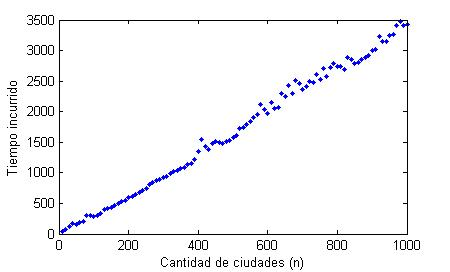
\includegraphics[scale=0.5]{imagenes/1-nosesalvanadie.jpg}
	\end{center}
	\caption{Zombieland - Ninguna ciudad salvada}\label{fig:1-nadie}
\end{figure}

Como en apariencia no podemos asegurar un comportamiento $n*log(n)$, decidimos dividir cada resultado de tiempo por la correspondiente cantidad de ciudades (Figura \ref{fig:1-nadie-n}) y por el logaritmo de esa cantidad (Figura \ref{fig:1-nadie-logn}).

\begin{figure}[htb]
	\begin{center}
    		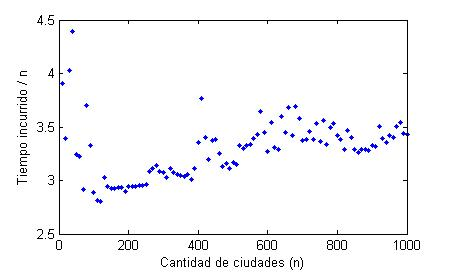
\includegraphics[scale=0.5]{imagenes/1-nosesalvanadie-div-n.jpg}
	\end{center}
	\caption{Zombieland - Ninguna ciudad salvada (div n)}\label{fig:1-nadie-n}
\end{figure}

\begin{figure}[htb]
	\begin{center}
    		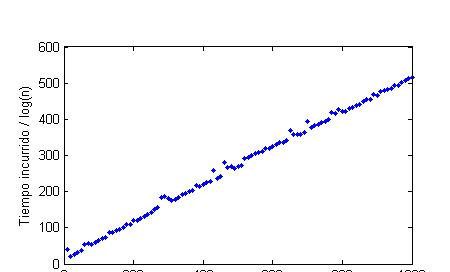
\includegraphics[scale=0.5]{imagenes/1-nosesalvanadie-div-logn.jpg}
	\end{center}
	\caption{Zombieland - Ninguna ciudad salvada (div log(n))}\label{fig:1-nadie-logn}
\end{figure}

Finalmente, dividimos los tiempos de ejecución por $n*log(n)$, siendo $n$ la cantidad de ciudades (Figura \ref{fig:1-nadie-nlogn}).

\begin{figure}[htb]
	\begin{center}
    		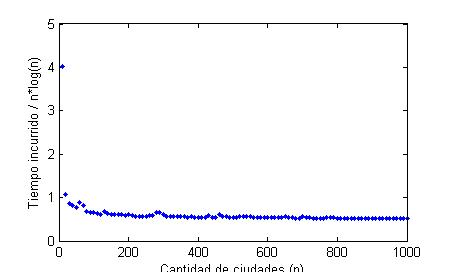
\includegraphics[scale=0.5]{imagenes/1-nosesalvanadie-div-nlogn.jpg}
	\end{center}
	\caption{Zombieland - Ninguna ciudad salvada (div n*log(n))}\label{fig:1-nadie-nlogn}
\end{figure}

Si bien el gráfico de la Figura \ref{fig:1-nadie} pareciera mostrar una recta, lo cual significaría que nuestro algoritmo sería $\mathcal{O}(n)$, y crecería linealmente, al observar la Figura \ref{fig:1-nadie-logn}, veo que al dividir por $log(n)$ queda algo parecido a una recta también, suceso que no debería ocurrir de ser $\mathcal{O}(n)$ nuestro algoritmo. Más aún, al ver la Figura \ref{fig:1-nadie-n} vemos la curvita inicial propia de la funcion $log(n)$, y para despejar cualquier duda, al dividir por $n*log(n)$, el gráfico de la Figura \ref{fig:1-nadie-nlogn} nos muestra que nuestra función tiende en tiempo a una constante. Es por eso, que estos gráficos parecerían respaldar la teoría de que nuestro algoritmo tiene complejidad $\mathcal{O}(n*log(n))$.

\vspace*{0.6cm}
%\newpage
\subsubsection{Test 2}

\vspace*{0.3cm}

Ahora veamos qué tanta incidencia tiene en el tiempo de ejecución, la cantidad de ciudades que se salvan.  Para ello, ejecutamos {\it Zombieland} con las mismas instancias aleatorias generadas anteriormente, pero esta vez con un presupuesto lo suficientemente grande como para que se salven todas las ciudades de cada país.

Nuevamente, se realizaron 50 ejecuciones para cada caso, se midieron los tiempos de ejecución, y se sacó el promedio para cada uno.  La Figura \ref{fig:1-comp} muestra en comparación los resultados de salvar a todas las ciudades y de no salvar a ninguna.

\begin{figure}[htb]
	\begin{center}
    		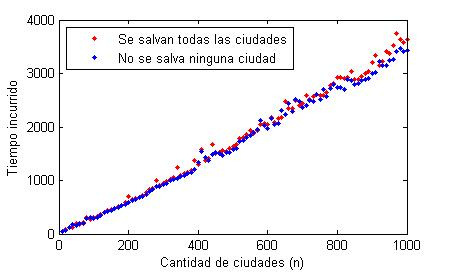
\includegraphics[scale=0.5]{imagenes/1-comparacion.jpg}
	\end{center}
	\caption{Zombieland - comparación de casos}\label{fig:1-comp}
\end{figure}

El gráfico pareciera respaldar nuestra teoría, puesto que podemos observar que los tiempos de ejecución son muy similares (al principio casi indistinguibles) con una leve inclinación a que no salvar a ninguna ciudad es más rapido que salvar a todas.

Por todo lo arriba experimentado, pareciera que nuestro material teórico tiene apoyo empírico.